\section{Implementation and Experiment Setup}
\label{sec:setup}

To evaluate the scalability of multithreaded programs in QEMU emulator, we 
setup QEMU with COREMU on a 48-processor AMD machine with Linux 2.6.32 running
on it. In QEMU, we setup a modified Debian for the only guest OS running. 
Benchmark applictions, Splash2 benchmarks and REDIS, are installed on both 
host OS and guest OS to obtain comparison result. 

\paragraph{QEMU\cite{rel:qemuwiki}}
QEMU stands for "Quick EMUlator" and is a processor emulator that relies on 
dynamic binary translation to achieve a reasonable speed while being easy to 
port to new host CPU architectures.
In conjunction with CPU emulation, it also provides a set of device models, 
allowing it to run a variety of unmodified guest operating systems; 
it can thus be viewed as a hosted virtual machine monitor. It also provides 
an accelerated mode for supporting a mixture of binary translation (for 
kernel code) and native execution (for user code), in the same fashion as 
VMware Workstation and VirtualBox. QEMU can also be used purely for CPU 
emulation for user level processes, allowing applications compiled for one 
architecture to be run on another.

\paragraph{COREMU\cite{rel:coremu}} 
QEMU itself doesn't support real multicore emulation 
(the multicore mode of QEMU actually runs all the virtual cores on a single 
physical core. To enable multicore support, we setup our experiment on 
\emph{COREMU}, an extension to QEMU to enable real multicore emulation. 

COREMU is a scalable and portable parallel full system emulator built on Qemu. 
Currently, COREMU supports x86\_64 and ARM (MPcore Cortex A9) target on x86\_64 
Linux host system. (Note that ARM support is not as stable as x86\_64 now.)
COREMU is able to boot 255 emulated cores running Linux on our testing machine 
which has only 4 physical cores (Intel Core(TM)2 Quad CPU Q6600, with 2G memory).

\paragraph{SPLASH-2 Benchmark Suite\cite{rel:splash2}}
SPLASH-2 is a collection of scientific parallel programs which are highly 
optimized and used to scalability testing. The benchmark suite is from the original
SPLASH benchmark suite, with some optimization and bug fixing. From SPLASH-2, 
we select 4 typical parallel programs:
\begin{itemize}
\item \emph{FFT}, which is short for Fast Fourier Transform, a widely used
algorithm in signal processing and other simple complex-number arithmetic. 
\item \emph{BARNES} and \emph{FMM}, which are two 3D simulation program for the 
interaction of human body and other objects.
\item \emph{OCEAN}, which is a simulation program for the large scale 
ocean movements and currents. 
\end{itemize}
Some evaluation and analysis of SPLASH-2 scalability can be found in the original
paper of SPLASH-2\cite{rel:steven}.

\paragraph{REDIS \cite{rel:redisweb}} 
Redis is an open source, advanced key-value store. 
It is often referred to as a data structure server since keys can contain strings, 
hashes, lists, sets and sorted sets. Redis provides a testing program which can be
used to measure the throughput of different operations for Redis server. From all
operatings provided in the test suite, we selected three of them for the purpose 
of scalability evaluation.
\begin{itemize}
\item PING: In this test, 50 clients are launched to ping the server process
multiple times and compute the frequency of ping operating returns.
\item SET: In this test, 50 clients are launched to put a random key-value pair
to the server process multiple times and compute the frequency of successful set 
operating. 
\item GET: In this test, 50 clients are launched to get a random key-value pair
from the server process multiple times and compute the frequency of successful get
operating. 
\end{itemize}

\subsection{Setup}

Here we're going to discuss the server setup and configuration, and the challenges
we met before the evaluation, including non-deterministic system clock and 
invalid logic networking devices.

\subsubsection{Server Setup}

We setup QEMU on an AMD server with Ubuntu running on it. The configuration is
as following:
\begin{itemize}
\item 6 cores (like this\cite{rel:amd6core} style) \\
48 processors (46 processors of 0.8GHz, 2 of 1.9GHz)
\item Cache size:
\begin{itemize}
\item index0: 64KB
\item index1: 64KB
\item index2: 512KB
\item index3: 5118KB
\end{itemize}
\item 64GB memory
\item Host Operating System: Linux 2.6.32-35-server
\end{itemize}

In QEMU emulator, we installed a debian image together with a Ubuntu kernel. 
\begin{itemize}
\item Cores and processors: depend on configuration
\item Cache size:
\begin{itemize}
\item index0: 32KB
\item index1: 32KB
\item index2: 4096KB
\end{itemize}
\item Depend on configuration
\item Host Operating System: Linux 2.6.32-220.el6.i686 + Linux 2.6.32-35-server
\end{itemize}

All the benchmark applications are installed in both the host operating system 
and the guest operating system with the same setup configuration. 
\begin{table}[h]
\center
\begin{tabular} {c|l}
Application & Configuration \\
\hline
FFT & $2^{24}$ size complex number array \\
FMM & Default data set \\
BARNES & Default data set \\
OCEAN & 258 size with contiguous simulation \\
REDIS & 50 clients 
\end{tabular}
\end{table}

\subsubsection{Cost Measurement}
System clock functions don't return exactly correct result in \emph{COREMU} 
because kernel implementation is modified slightly to enable multicore support.
Therefore, taking system clock to measure program performance, which is used in
SPLASH-2 and Redis, is unreasonble. In order to obtain precise result in COREMU,
we replaced all the performance measurement code in COREMU and Redis with 
CPU cycle counter. 

\paragraph{SPLASH-2} SPLASH-2 benchmarks share a common source for performance 
measurement. 
We replaced this part of code (as showed in figure\ref{fig:cyclecounter}). 
The original implementation uses \texttt{gettimeofday} to obtain current clock, 
which is non-deterministic due to the kernel clock simulation. In the new 
implementation, we use \texttt{rdtsc} to obtain CPU cycle counter and use it
for system clock. 
\begin{figure}[H]
\center
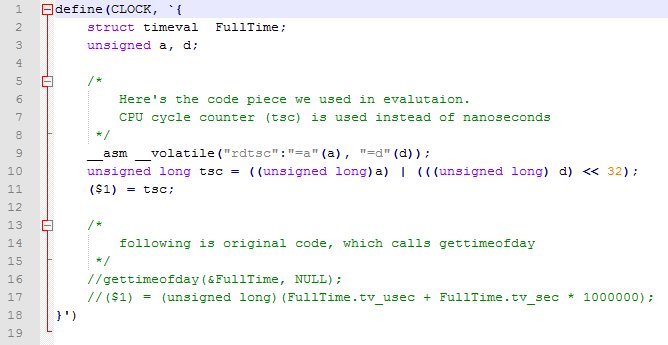
\includegraphics[width=0.8\linewidth]{figures/cycle_counter_codes.png}
\caption{Performance measurement codes in SPLASH-2}
\label{fig:cyclecounter}
\end{figure}

\paragraph{Redis}
Redis benchmark program uses the formula
\begin{equation}
Throughput = \frac{\# \ of \ requests\ processed}{Time\ consumption}
\end{equation}
to obtain throughput of a bunch of operations. To prevent the non-determinism 
in the computation of \emph{Time consumption}, we replace the time argument 
with CPU cycles simular to SPLASH-2. In this way Redis will output the throughput
based on unit CPU cycle.

\subsubsection{Network Access}

The debian image running on COREMU doesn't have a working network component.
This defect prevents us from synchronizing data between host OS and guest OS.
The debian image, however, is the only image that can be correctly supported by 
COREMU. In order to setup network access in the debian image, we installed a 
Ubuntu kernel in the same image. The Ubuntu kernel, allows network connection 
to be established when the orignal QEMU is used for emulation. 

\begin{table}[H]
\center
\begin{tabular} {c|c|c}
 & Debian Kernel & Ubuntu Kernel \\
\hline
QEMU & No network, no multicore & Nework, no multicore \\
COREMU & No network, multicore & Crash
\end{tabular}
\caption{Network Access and Multicore Support}
\end{table}

\subsection{Hypothesis}
To reason about the scalability problems which are only present in the
virtualized environment, we investigated the design and implementation
of the QEMU virtual machine, and the COREMU system, and proposed some
possible hypothesis for the scalability problems:

\begin{itemize}
	\item Atomic operations between virtual cores may be more expensive
		than the same operations between real cores.\\
		Atomic operations require extra work to keep the results correct.
		In real systems, these works are usually done by the hardware.
		Most architectures have specific atomic instructions to perform
		atomic operations. In the virtualized envrionment, hardware is
		emulated by the virtual machine monitor. In this case, emulating
		atomic instructions may be expensive, since this requires
		inter-thread communications and synchronizations.
	\item Scheduling virtual cores onto real cores and migrating them
		between different cores may incur extra overhead. \\
		Virtual machine monitors need to map virtual cores onto real cores.
		They use scheduling algorithms to decide which virtual cores should
		be mapped to each real core. If the scheduling algorithm is not
		correctly designed, it may cause slowdown. For example, if the
		virtual machine monitor migrates virtual core from one real core
		to another frequently, it would have huge impact on the performance,
		since the cache would be flushed frequently, and data needs to be
		reloaded when being used on a new core.
	\item Communication between virtual cores may be harder to scale
		than communication between real cores. \\
		In the native environment, inter-core communications are implemented
		through Inter Processor Interrupts(IPIs), shared-memory accesses,
		and other methods. To keep the cache coherent, cache coherence
		protocols are usually run between caches in different cores. In
		the virtualized environment, all these methods need to be implemented
		in the virtual machine monitor. Although shared-memory accesses may
		not be affected, other methods may have significant overhead.
\end{itemize}

